\documentclass[11pt]{article}
\usepackage[utf8]{inputenc}
\usepackage{amsmath, amssymb}
\usepackage{graphicx}
\usepackage{hyperref}
\usepackage{geometry}
\usepackage{cite}
\usepackage{listings}
\usepackage{subcaption}
\usepackage{tabularx}

% Geometry settings
\geometry{a4paper, margin=1in}

% Title and author
\title{Planar Cable-Driven Robot}
\author{Arzaq Khan \\
Hamdan Raashid \\
}
\date{\today}

% Code block settings
\lstset{
  basicstyle=\ttfamily\small,
  breaklines=true,
  frame=single,
  numbers=left,
  numberstyle=\tiny,
  xleftmargin=2em,
  language=Python % Change as needed
}

\begin{document}

\maketitle

\section{Introduction}
\subsection{Project Description}
Our project is a planar cable-driven driven that continously tracks and follows objects in real time. If we had been able to
implement everything according to our initial plan, we would have been able to apply the robot in a logistics setting to pick and
place objects. Unfortunately, due to certain problems we encountered, which is discussed in a later section, we were unable to
strictly follow our original plans.

During the planning stage, we aimed to design a planar cable-driven robot that would pick a user selected target and drop off that
target to a user selected location. The user would first select the target in a video feed provided by a staionary camera and the
robot would move the end-effector to where the target is located. Next, a command would be given to the end-effector to switch on the
electromagnet to pick up the target. Then, the user would provide a location to drop off the target using
the same video feed and the robot would drop off the target at said location. 
Although our actual robot is similar to what we had planned initially, there are slight differences.

The main difference between what we built and we had planned lies in the parts we used and the end-effector. We had
planned to use an ESP32, a microcontroller, for its Bluetooth and WiFi features and stepper motors due to their precision.
Unfortunately, we could not get the stepper motors to work. We initially figured that it was a power issue, but even
after connecting the motors to an external power supply, we could not get the motors to move. As for the end-effector,
we could not mount an electromagnet on it due to issues discussed in a subsequent section. To summarize, what we have
is a robot that can continously track and follow objects, but cannot pick them up.

\begin{figure}[h!]
\centering

\begin{subfigure}[b]{0.3\textwidth}
    \centering
    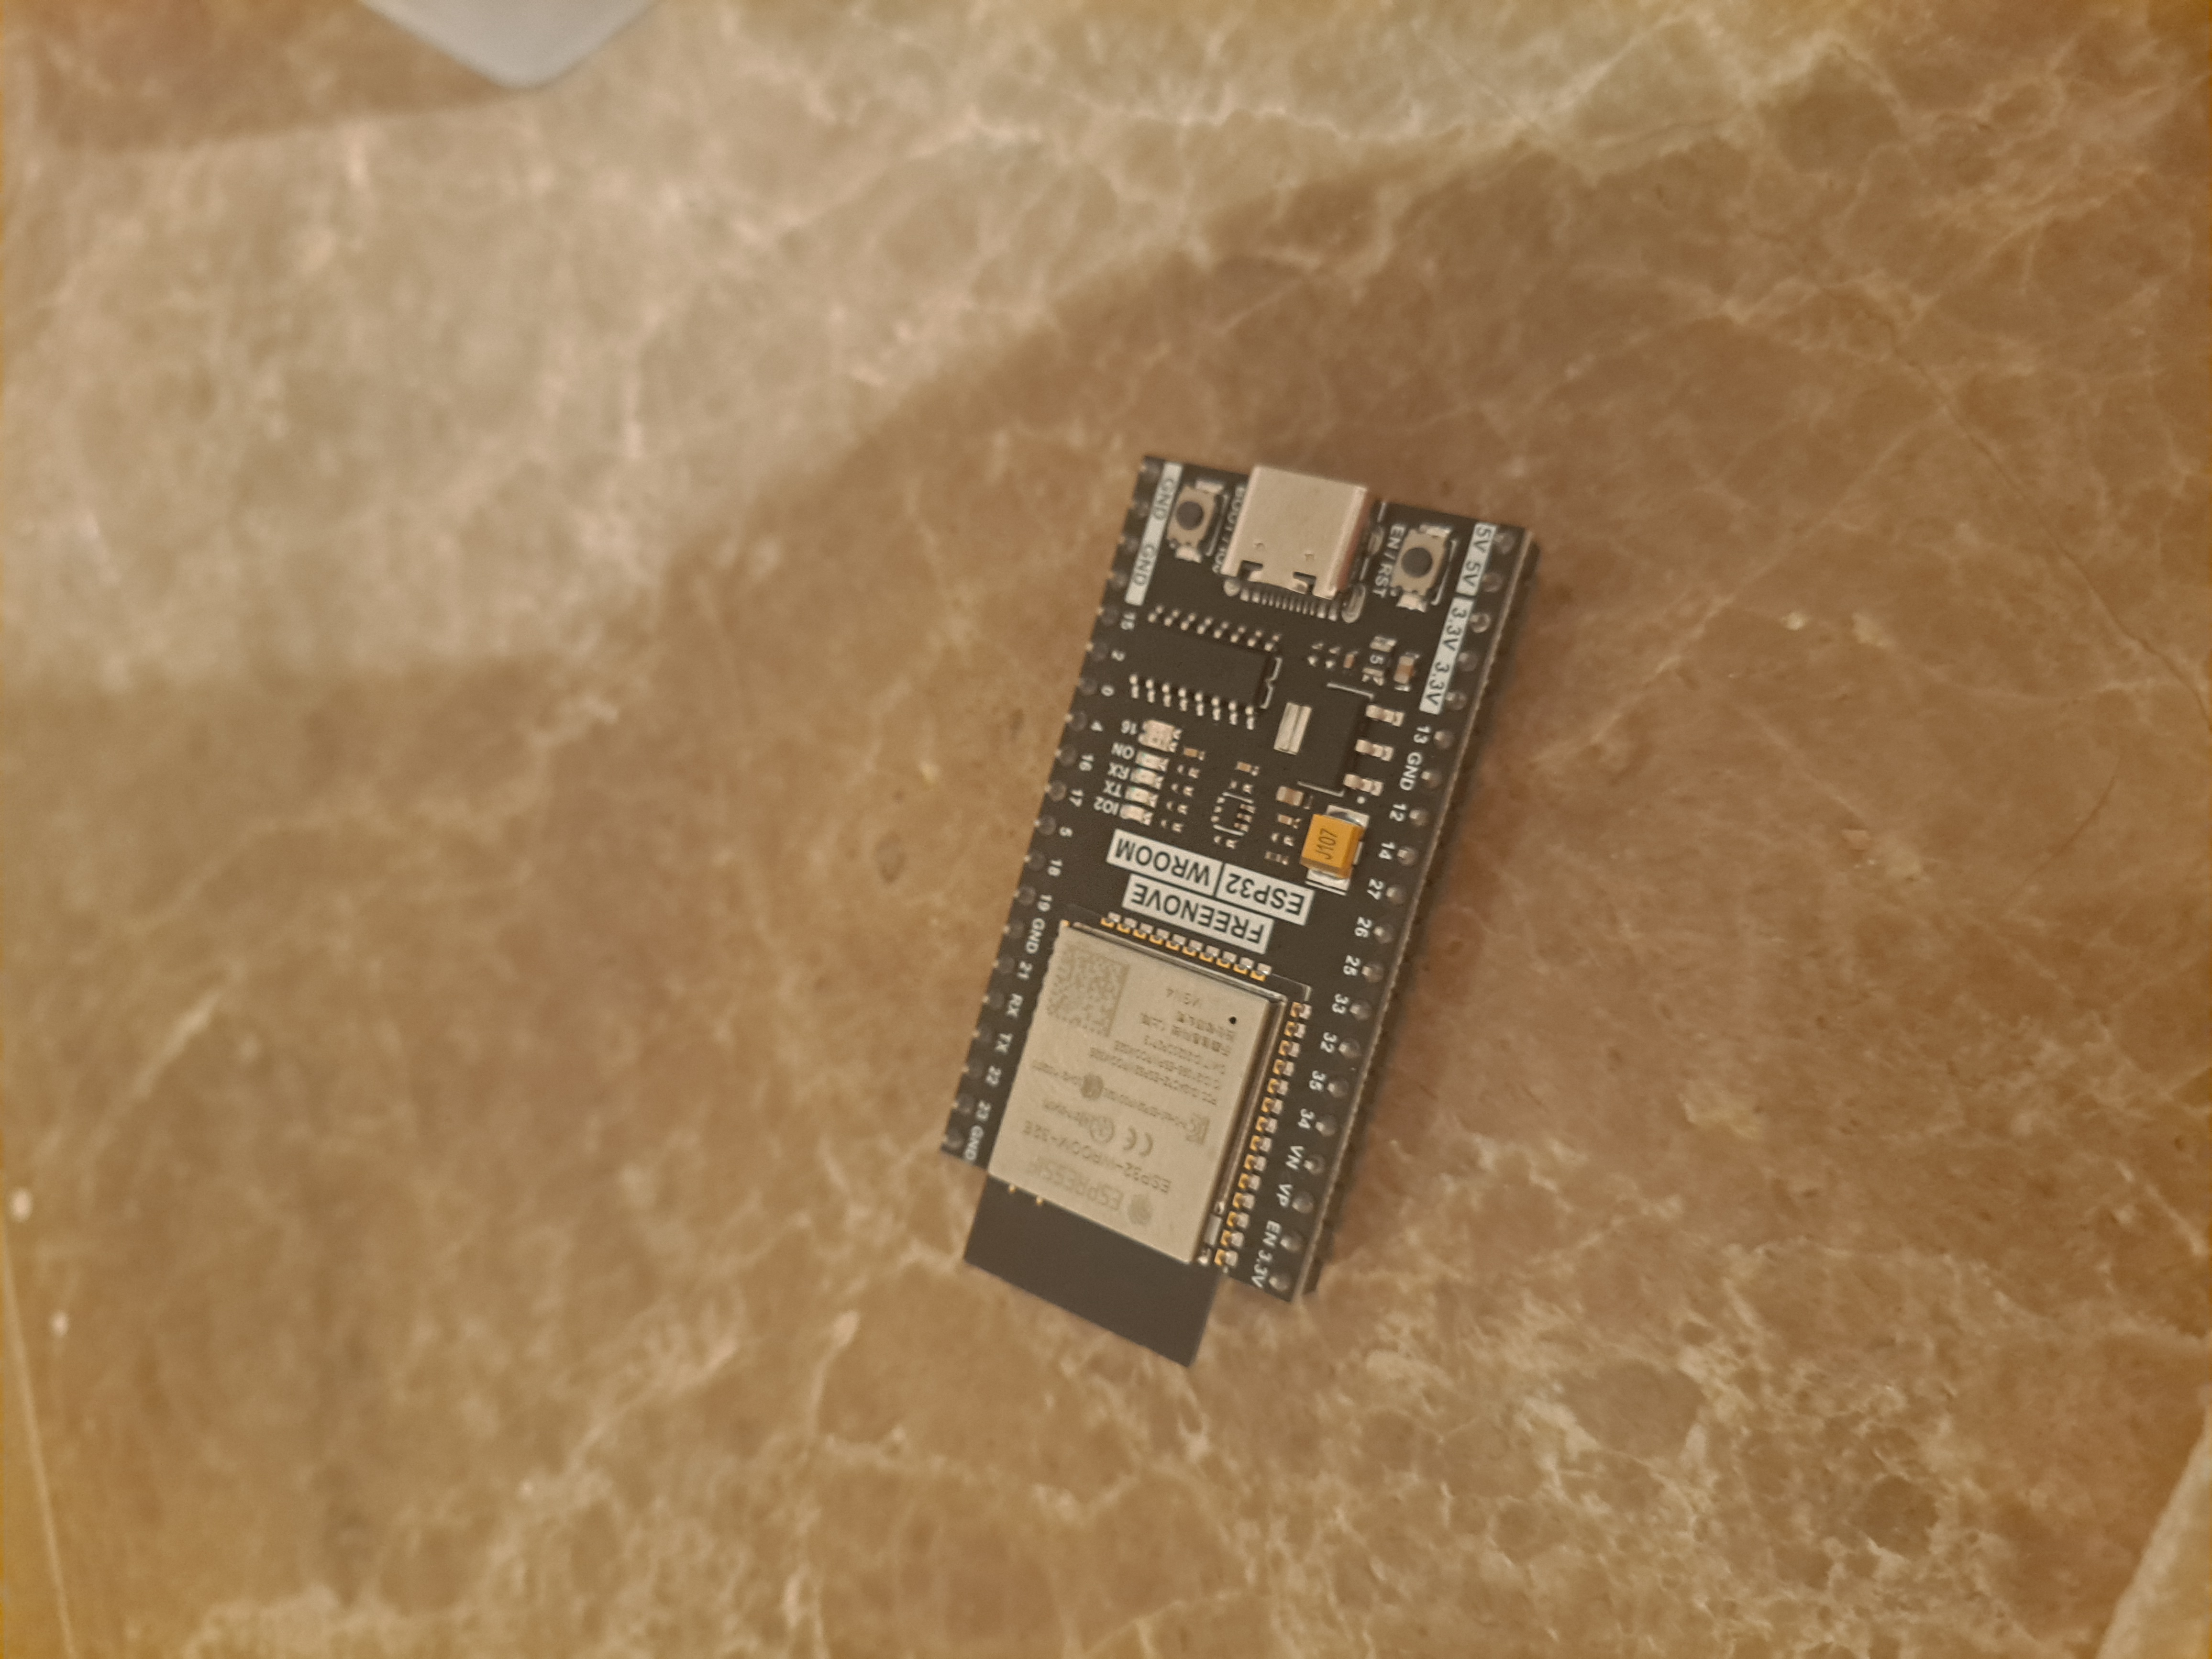
\includegraphics[width=\textwidth]{ESP32Img.jpg}
    \caption{An ESP32 microcontroller.}
    \label{fig:figure1}
\end{subfigure}
\hfill
\begin{subfigure}[b]{0.3\textwidth}
    \centering
    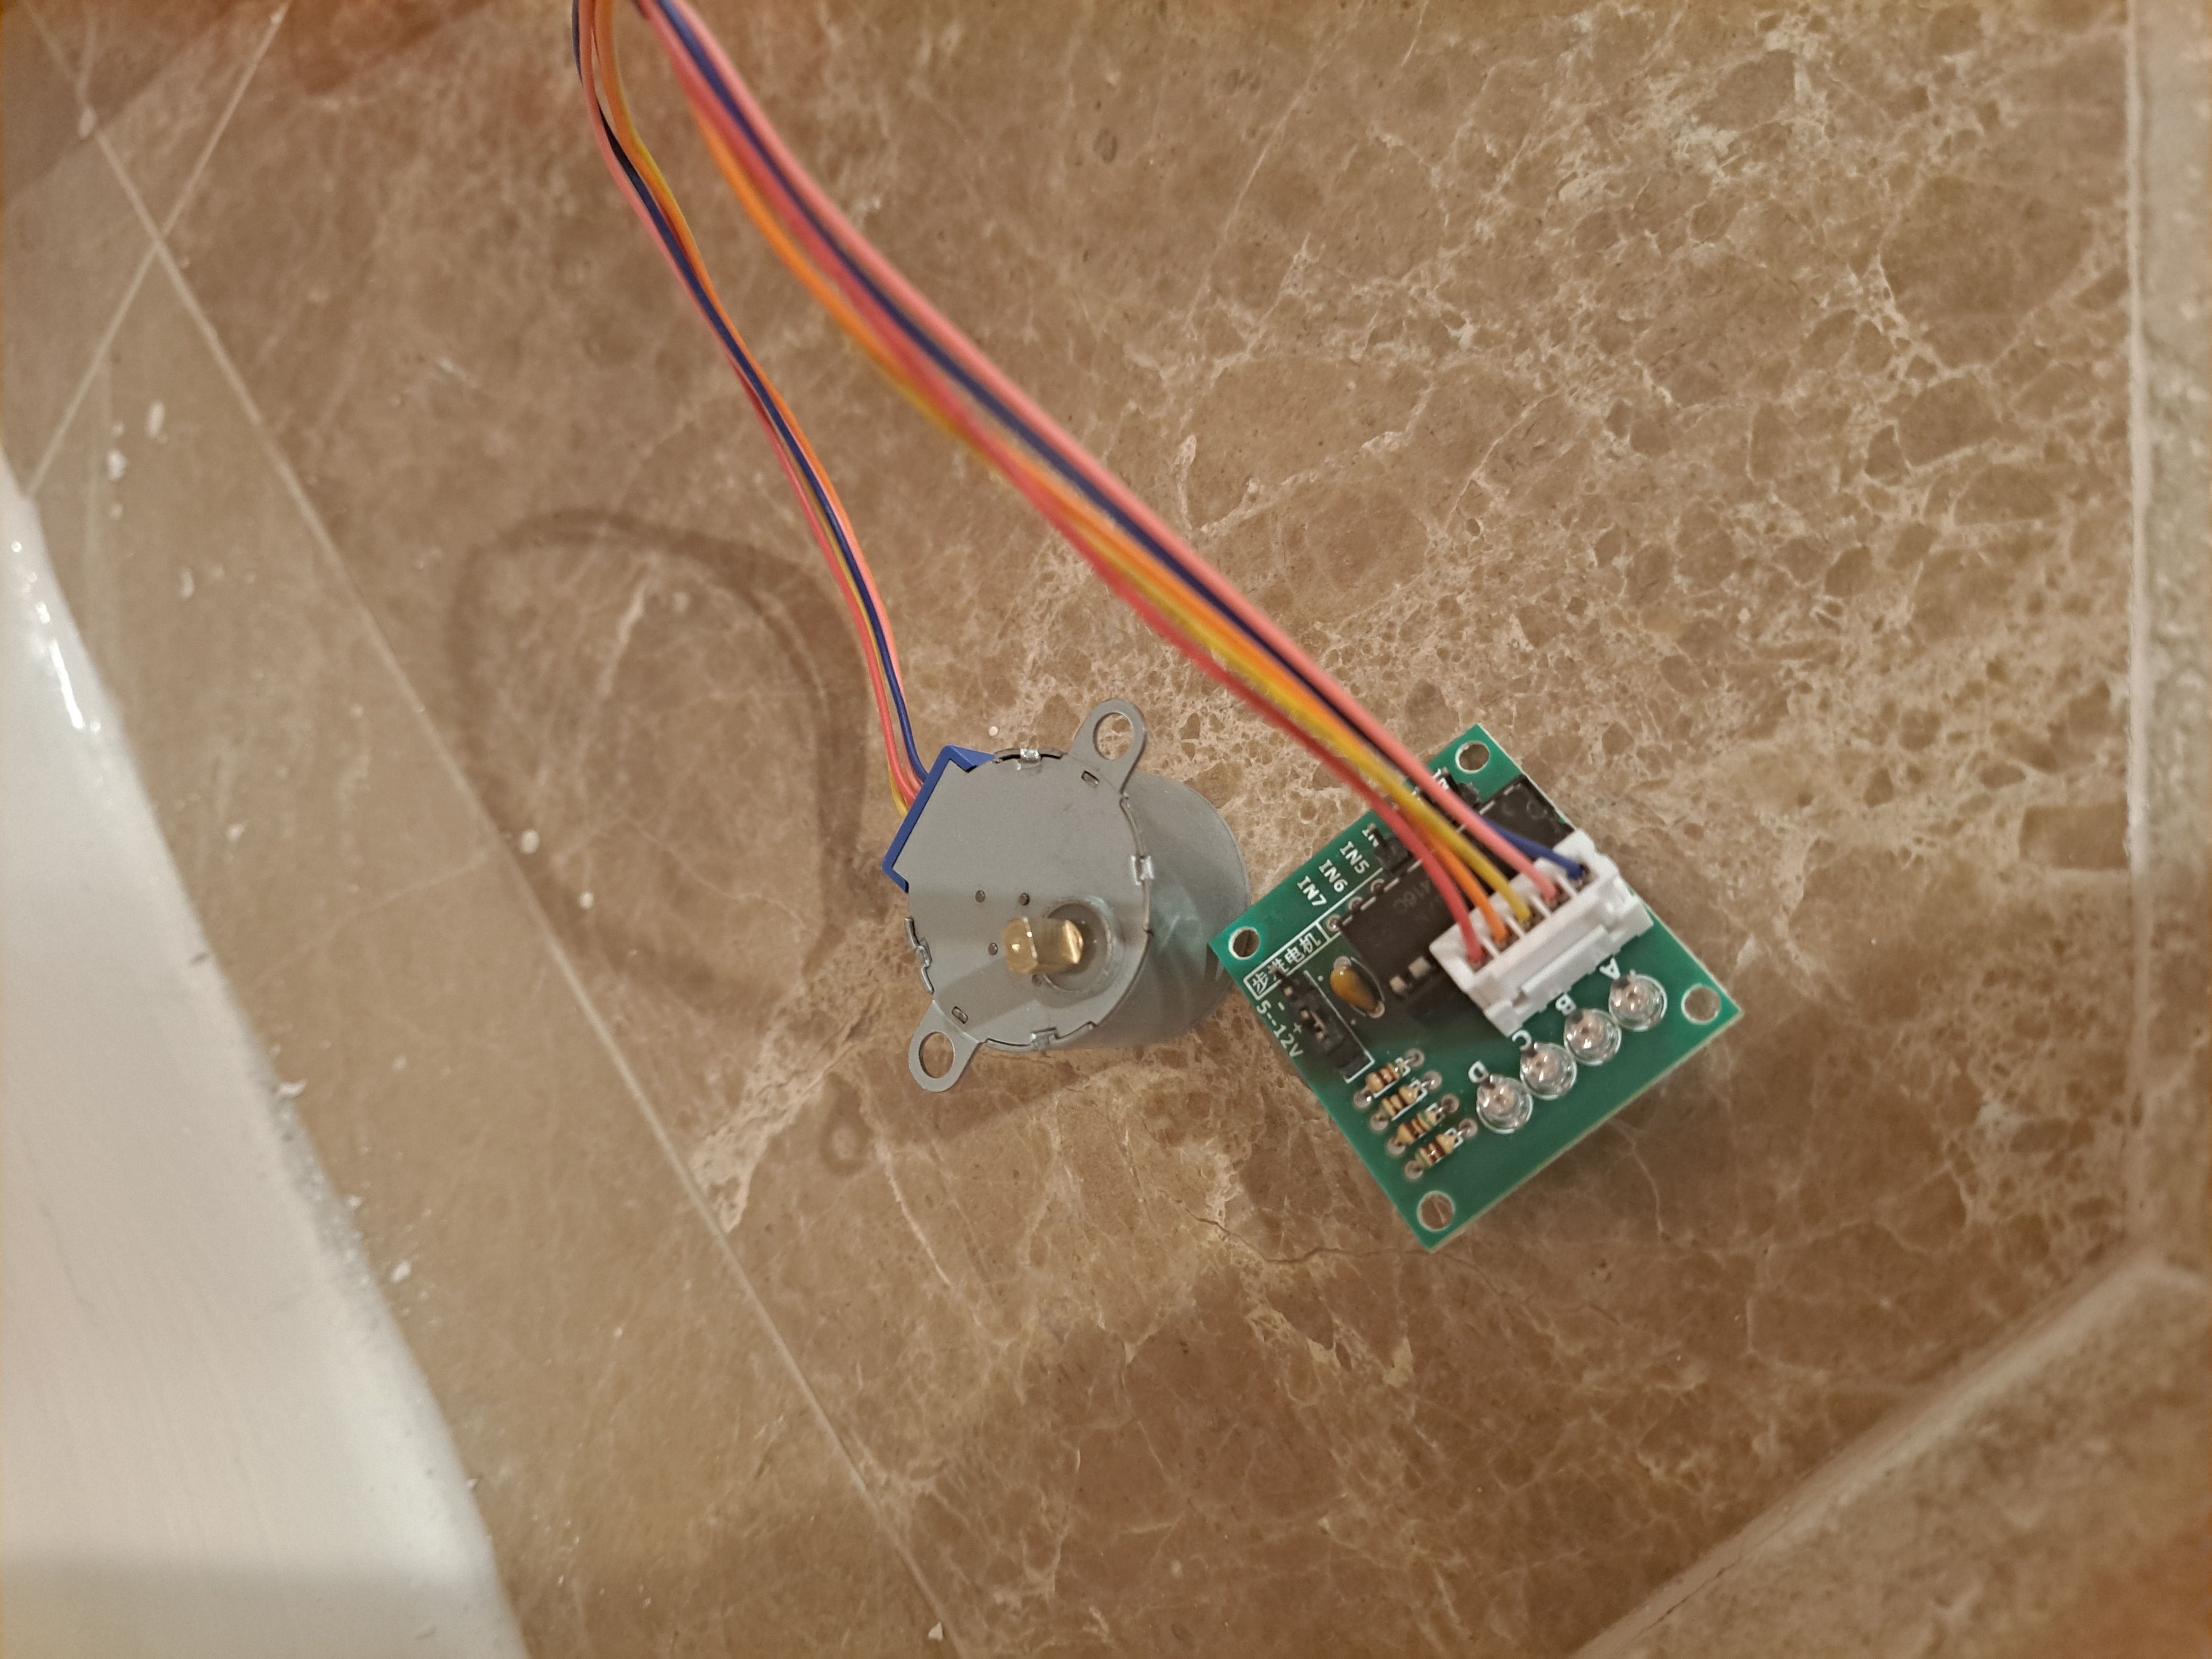
\includegraphics[width=\textwidth]{MotorImg.jpg}
    \caption{A stepper motor.}
    \label{fig:figure2}
\end{subfigure}
\hfill
\begin{subfigure}[b]{0.3\textwidth}
    \centering
    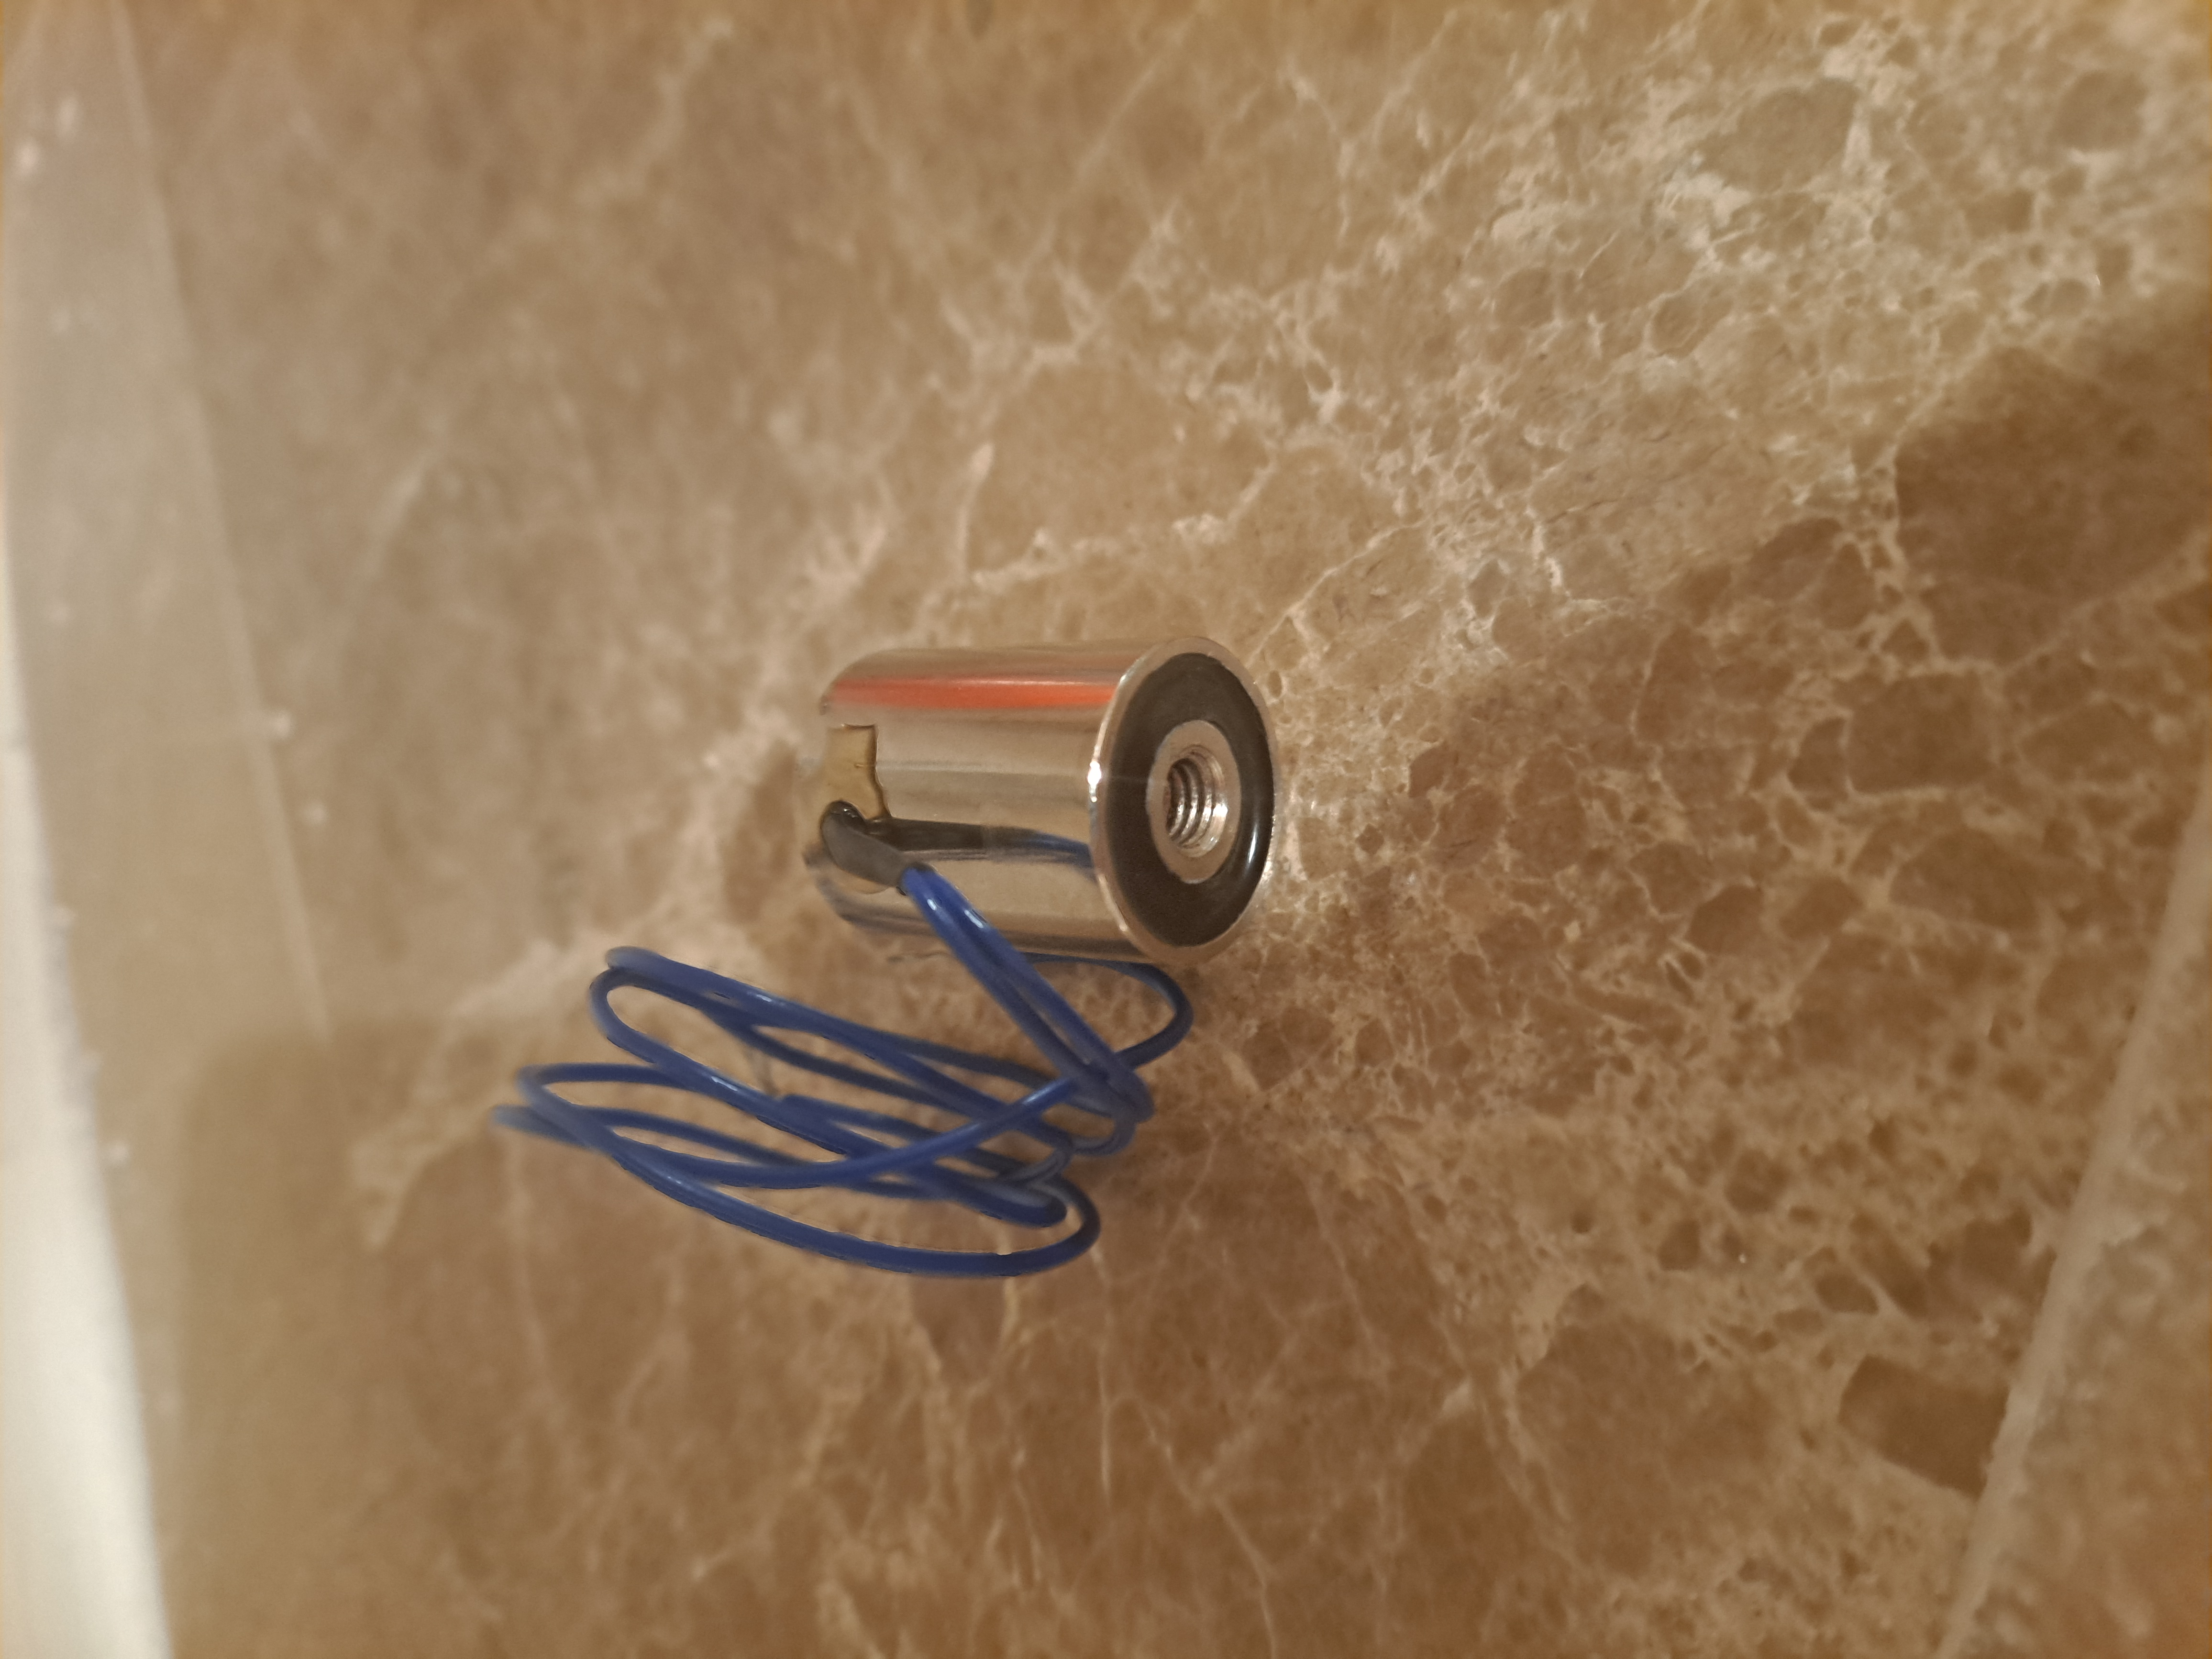
\includegraphics[width=\textwidth]{ElectromagnetImg.jpg}
    \caption{An electromagnet.}
    \label{fig:figure3}
\end{subfigure}

\caption{Three side-by-side figures showing an ESP32, a stepper motor, and an electromagnet.}
\label{fig:side_by_side}
\end{figure}
  


\subsection{Introduction to Cable-Driven Robots}
A cable-driven robot is actuated using cables. The main parts of a cable-driven robot include winches, cables, motors, and 
a mobile platform/end-effector. The active length of the cables are controlled by the winches, and this is what determines the position of
the end-effector. Changing the active length of the cables changes the position of the end-effector.

\begin{figure}[h]
\centering
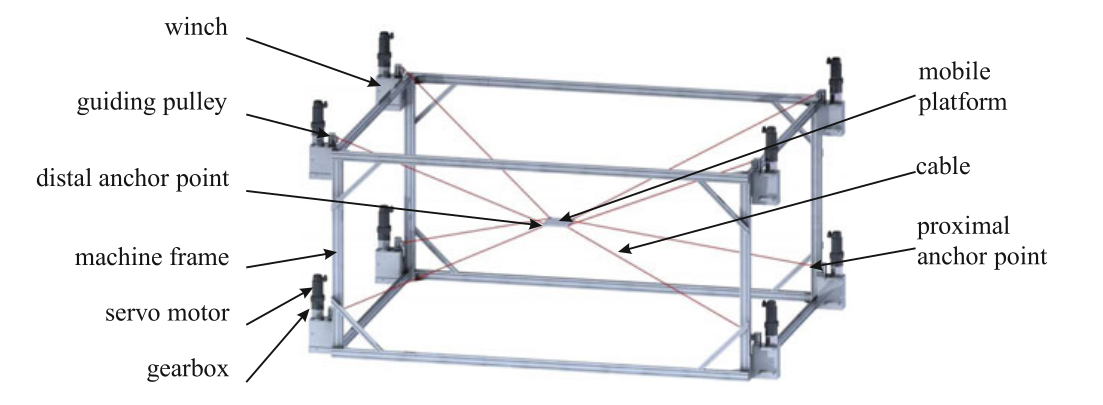
\includegraphics[width=0.5\textwidth]{Cabledrivenrobot.png}
\caption{A cable-driven robot from \cite{pott2018cable}.}
\label{fig:figure6}
\end{figure}

Cable-driven robots offer one main advantage over serial robots: they are light weight. This is because, unlike the serial case, the
motors do not have to bear the weight of other motors. Therefore, much higher speeds can be achieved. 

\section{Methodology}
\subsection{Inverse Kinematics Model}
The inverse kinematics model for the robot determines the required cable lengths to achieve the desired position of the end effector. The derivation assumes a fixed base frame and utilizes geometric relations between the pulley positions and the end-effector's coordinates.
\begin{figure}[h]
\centering
\includegraphics[width=1\textwidth]{InverseKinematics.jpg}
\caption{Inverse Kinematics Reference Diagram}
\label{fig:robot}
\end{figure}
\subsubsection*{Cable Length Calculation}

Let the system frame be defined by four points: \( A (0, 60) \), \( B (60, 60) \), \( C (60, 0) \), and \( D (0, 0) \). The center of the end effector is initially located at \( O(O_x = 30, O_y = 30) \). The coordinates of the edges of the end effector (points \( P, Q, R, S \)) are calculated with respect to this center as follows:

\[
P = \begin{bmatrix}
O_x - 2\\
O_y + 3
\end{bmatrix}, \quad
Q = \begin{bmatrix}
O_x + 2\\
O_y + 3
\end{bmatrix}, \quad
R = \begin{bmatrix}
O_x + 2\\
O_y - 3
\end{bmatrix}, \quad
S = \begin{bmatrix}
O_x - 2\\
O_y - 3
\end{bmatrix}
\]

\vspace{0.2cm}
\noindent
For a given end-effector center position, the cable lengths associated with each (motor - end-effector edge) pair are given by:

\[
L_{A} = \| P - A \|, \quad
L_{B} = \| Q - B \|, \quad
L_{C} = \| R - C \|, \quad
L_{D} = \| S - D \|
\]

\vspace{0.2cm}
\noindent
Therefore, to move the end-effector center from point 1 to point 2, we calculate the corresponding cable lengths for the two states, and then the absolute difference between the two.

\[
\Delta L_{A} = \left| L_{A_{\text{new}}} - L_{A_{\text{old}}} \right|, \quad
\Delta L_{B} = \left| L_{B_{\text{new}}} - L_{B_{\text{old}}} \right|
\]
\[
\Delta L_{D} = \left| L_{D_{\text{new}}} - L_{D_{\text{old}}} \right|, \quad
\Delta L_{C} = \left| L_{C_{\text{new}}} - L_{C_{\text{old}}} \right|
\]

\subsubsection*{Motor Control Logic}

The motor movement in the system is defined by three parameters: the control action required, the velocity of the motor, and the angle by which it should move. Let motors A,B,C and D (the names corresponding to their positions on the system frame) be generally referred to as X.

\vspace{0.2cm}
\noindent
To determine the control action for each motor:
\begin{itemize}
    \item If \( L_{\text{new}} > L_{\text{old}} \): Release cable (push)
    \item If \( L_{\text{new}} < L_{\text{old}} \): Contract cable (pull).
\end{itemize}

\noindent
The change in angle (in radians) required for each motor, with a pulley with radius r attached to it is calculated as:
\[
\Delta \theta_{X} = \frac{\Delta L_{X}}{\text{r}}
\]

\noindent
The motor velocities are derived in the next section. By running the motors concurrently and setting variable velocity to handle each of the cable difference, the system minimizes total operation time while ensuring synchronization.

\subsubsection*{Constant Time - Variable Motor Velocity}

To ensure smooth motion, a constant-time approach is used instead of constant velocities for all the motors. Fixing the cable velocity of the motor that handles the largest cable change, the velocities of the other motors are proportionally scaled down.

\[
v_i = v_{\text{max}} \cdot \frac{\Delta \theta_x}{\Delta \theta_H},
\]

where \( v_{\text{max}} \) is the velocity of the motor handling the largest change in cable length, \(\Delta \theta_H \) represents the largest change in angle required among the four motors to move to the desired position and \( \Delta \theta_x \) represents the change in angle required in each motor X.
\vspace{0.2cm}
\noindent
The time required for all motors is equal:
\[
t = \frac{\Delta \theta_H}{v_{\text{max}}}.
\]
\noindent
This approach ensures all motors complete their movement simultaneously, reducing cable slack and ensuring smooth operation of the robot.

\subsection{Planar Homography}

Since the camera does not have an overhead view of the workspace, the relationship $(x, y) = s(u, v)$ does not hold. Here
$(x, y)$ is the physical coordinate, $s$ is a scale factor, and $(u, v)$ is the pixel coordinate. There is a linear
relationship between the pixel coordinates and physical coordinates in plane described by a homography matrix. The homography
matrix is invertible, because unlike the general case where we a translating between a 3D point in space and a pixel in a 2D image,
we are translating between a 2D plane in reality and a 2D pixel space. The homography matrix has 8 degrees of freedom, $h_1, \dots, h_8$.

$$ H =
\begin{pmatrix}
h_1 & h_2 & h_3 \\
h_4 & h_5 & h_6 \\
h_7 & h_8 & 1 \\
\end{pmatrix}
$$

Let $X_1, X_2, X_3, X_4$ be four points on a physical plane in homogeneous coordinates and $x_1, x_2, x_3, x_4$ the corresponding pixel coordinates in homogeneous form.
Then the following equations:

\begin{align*}
X_1 &= Hx_1 \\
X_2 &= Hx_2 \\
X_3 &= Hx_3 \\
X_4 &= Hx_4
\end{align*}

define a system of linear equations, which can be solved for $h_1, \dots, h_8$. This is why there is a calibration phase before the robot starts moving. Now
say there is a point on the video feed, $p$, whose physical coordinate is needed. Applying the homography matrix on the pixel coordinate, $P = Hp$, we get
$P$, the physical coordinate corresponding to $p$.

\subsection{Vision}
We used OpenCV for object tracking and everything related to computer vision. More specifically, we used OpenCV's CSRT
tracker. The figure below shows the control flow for the vision system.

\begin{figure}[h]
\centering
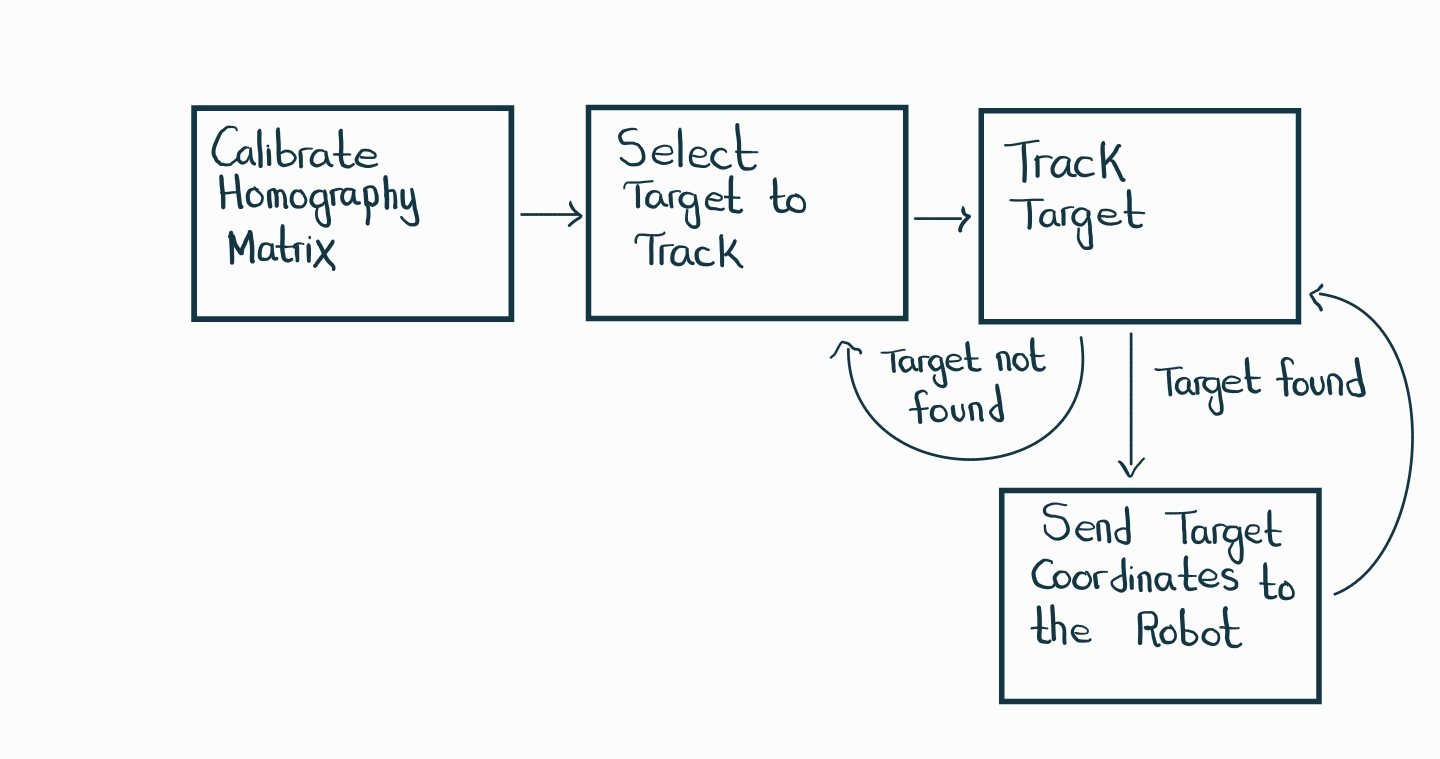
\includegraphics[width=0.5\textwidth]{VisionSystem.jpg}
\caption{Control flow for the vision system.}
\label{fig:figure4}
\end{figure}

First, marked points are selected in the video
feed to calibrate the homography matrix. Next, the user selects the target to be tracked. Depending on whether OpenCV
successfully tracks the object in the most recent frame, the path diverges into two. If the tracking fails, the user has
to select the target again. If the tracking is successful, the server sends the physical coordinates to the EV3 and continues
to track the target.


\section{Results}
To evaluate the performance of the robot, three distinct tests were conducted, each focusing on a specific aspect of the system's movement and precision.
\subsection{Test 1: Continuous Motion Evaluation}
This test involved moving the end effector through a continuous motion between four predefined points. The experiment was conducted at varying velocities across different trials to assess the robot's capability to maintain smooth and accurate movement under dynamic conditions. The following table summarizes the results obtained from the robot's movement tests at different maximum speeds. The tests involved moving the end effector (EE) to four predefined points, with the accuracy of the robot's movement being evaluated at each speed. \newline
\noindent
The actual pre-defined points are (30.5, 45.5), (45.5, 30.5), (30.5, 15.5), (15.5, 30.5).

\begin{table}[h]
\centering
\begin{tabularx}{\textwidth}{|c|X|}
\hline
\textbf{Max Speed} & \textbf{Found Points} \\
\hline
30  & (30.7, 45.0), (45.7, 29.2), (30.7, 14.5), (16.4, 30.2) \\
\hline
50  & (30.5, 46.0), (45.0, 30.4), (30.3, 15.0), (16.5, 30.0) \\
\hline
70  & (30.0, 47.0), (44.0, 29.5), (29.7, 15.2), (15.5, 29.9) \\
\hline
\end{tabularx}
\caption{Test results for different maximum speeds and end effector movement accuracy.}
\label{tab:test_results}
\end{table}

\begin{figure}[h]
\centering
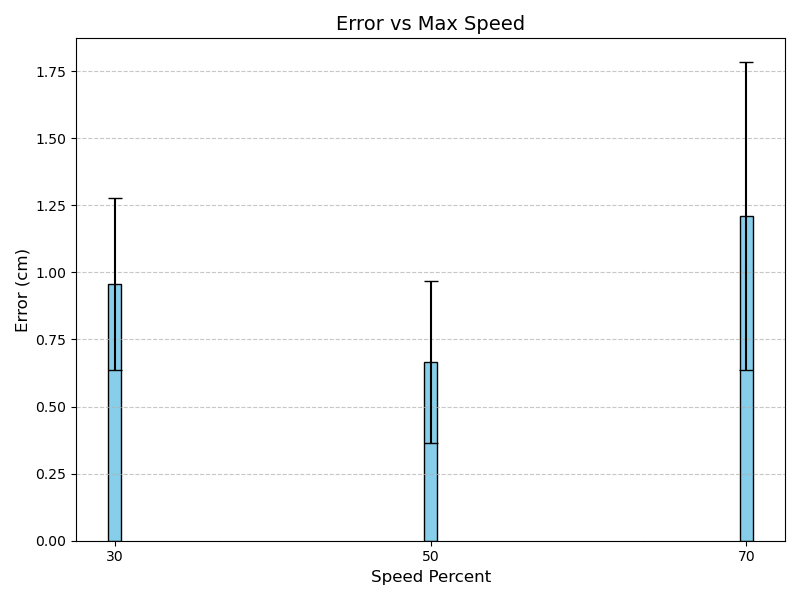
\includegraphics[width=0.6\textwidth]{Cont_motion_graph.png}
\caption{A temporary error graph.}
\label{fig:figure5}
\end{figure}

\subsection{Test 2: Repeatability Test}
The aim of this test was to evaluate the robot's repeatability in reaching a specific target location. The robot was commanded to move to a randomly chosen point, \((23, 19)\), three times. For each trial, the error was calculated as the difference between the desired target position and the actual position reached by the robot. The repeatability of the system was then assessed based on the magnitude and consistency of these errors.

\begin{table}[h]
\centering
\begin{tabularx}{\textwidth}{|c|c|X|}
\hline
\textbf{Trial} & \textbf{Displacement (x, y)} & \textbf{Norm Difference (Expected - Observed)} \\
\hline
1 & (+0.4, -0.7) & 0.81 \\
\hline
2 & (+0.0, -0.6) & 0.60 \\
\hline
3 & (+0.2, -1.3) & 1.31 \\
\hline
\end{tabularx}
\caption{Repeatability test results showing the displacement values and the norm differences.}
\label{tab:repeatability_test_norm}
\end{table}

\newpage
\subsection{Test 3: Homography Matrix Validation}
The Homography matrix, used to map pixel coordinates to physical coordinates, was validated through this test. Four physical points were recorded, and their corresponding pixel coordinates were transformed using the Homography matrix. The test evaluated the accuracy of the transformation by comparing the computed physical coordinates with the actual recorded physical points.
The average error produced by the homography transformation is 1.72 (measured using the norm of the difference).
\begin{table}[h]
\centering
\begin{tabular}{|c|c|}
\hline
\textbf{Actual Coordinates} & \textbf{Homography Coordinates} \\
\hline
(30.5, 45.5) & (31.00, 44.68) \\
\hline
(45.5, 30.5) & (45.03, 28.58) \\
\hline
(30.5, 15.5) & (29.49, 13.45) \\
\hline
(15.5, 30.5) & (15.13, 28.90) \\
\hline
\end{tabular}
\caption{Comparison of Actual Coordinates and Homography Coordinates.}
\label{tab:coordinates_comparison}
\end{table}

\section{Discussion}

\subsection{Errors}
We expected the errors to increase as the max speed was increased, just like it's the case for mobile rovers and serial robot arms. 
However, the data does not support this. Increasing the max speed did not have a significant effect on the accuracy of the 
cable-driven robot. The math explains why this is the case.

Increasing the speed causes inaccuracies with the motor angles. Suppose the error in the motor angle is $\alpha$ degrees. In
radians that would be $0.017\alpha$. Since the radius of the winches is 2cm, the error in the cable length is going to be
$2 \cdot 0.017\alpha$. As an example, taking the error in the motor angles to be 10 degrees, the error in the cable is only
going to be 0.34 cm.

Analyze and interpret the results. Discuss their implications, limitations, and potential future work.
Could talk about why the end-effector could not be done here.
Remember to discuss the pulley problem. Using Lego connector pins as pulleys causes problems. We 3D printed pulleys
but they would slip. Limitations with the 3D printer precision. Also in the discussion should be why the error
values for the end-effector position are so low. Also should be talked about sources of error.
It's a planar robot, which means that it cannot exert force perpendicular to the plane. If weight is added to the end-effector
there is no way the robot can counteract that force. Which will cause the cables to bend. There is a mechanism we thought
about but did not have the time to implement. Compare the precision of the cable-driven robot with the lab2 robot arm that was
made using the same components. Another thing to include: why Broyden's method could not be used. If the jacobian is not
perfect, incorrect changes in the cable lengths would break the system.

\section{Conclusion}
Summarize the key findings and their significance. Suggest directions for further research (tension model?).


\bibliographystyle{plain}
\bibliography{references}

\appendix
\section{Appendix: Additional Details}
\subsection{Setting Up Scrcpy and OBS Studio}
Install Scrcpy, and OBS Studio in your laptop, follow these steps:
\begin{enumerate}
    \item Enable USB Debugging on your phone under \texttt{Settings > Developer Options}.
    \item Connect your phone to the computer via USB.
    \item Run \texttt{scrcpy} in the terminal to mirror the phone's screen to the computer.
    \item In OBS Studio, Start Virtual Camera after adding scrcpy source.
\end{enumerate}
This setup allows you to use your phone as an external camera in the code.

\subsection{Working Directory Setup}
\begin{verbatim}
src/
|-- ev3-client/                         
|   |-- sample_client.py               Client Code for performing Visual Tracking
|   |-- System_constT.py               Attributes and Functions for using System
|   |-- System_InverseKinematics.py    Client Code for running direct Inv. Kin. Motion
|-- vision-server/
    |-- myenv/
    |-- vision_server                  Code for doing Homography fn. computation
\end{verbatim}
\end{document}